\chapter{Details}\label{chap:details}
\section{Path Following and Potential Fields}
While developing our search algorithms in the last lab we realized that doing full $A*$ searching was not going to be possible in ruby if our discretization was too granular. To alleviate this problem Duane Johnson developed a small library written in C which acted as a module to the rest of our code.  We also simplified the representation of the discretized map for the algorithm to search through.  With these changes we were able to search through maps of 80x80 in approximately 1/10 of a second.  This was fast enough and granular enough for the purpose of finding our way through a maze and deploying a decoy-sniper tactic.
\par
When it came time to follow the solution path returned by Duane's $A*$ module the immediate thought was to use potential fields along the length of the path.  The potential fields code developed in the first lab already had a PD controller which would suggest velocity and angular velocity based on the current position and angle of the tank.  As the lab progressed we optimized this algorithm to actually look as far ahead as the line segments are parallel so that when driving in a straight line we don't spend much time re-evaluating the path.  We also periodically re-evaluate the search solution which will be important in the future when we are trying to avoid enemy tanks and our world becomes more dynamic.
\par
In addition to the path following optimizations we also 'tuned' the relative strength of the fields and their radii so that as we approach the next Potential Field the system will move it to the next location before our arrival.  This helped to avoid uneccesary 'braking' and turning.

\section{Tests with Another Group}
\subsection{Our Tests}
We ran the tests for our implementation on the astar.bzw map from the lab website. Our tests went well with the exception of the return trip to our base after capturing the flag.  This is the one odd behavior for which no solution has yet been found.
\par
\begin{figure}\label{fig:stuck}
\begin{center}
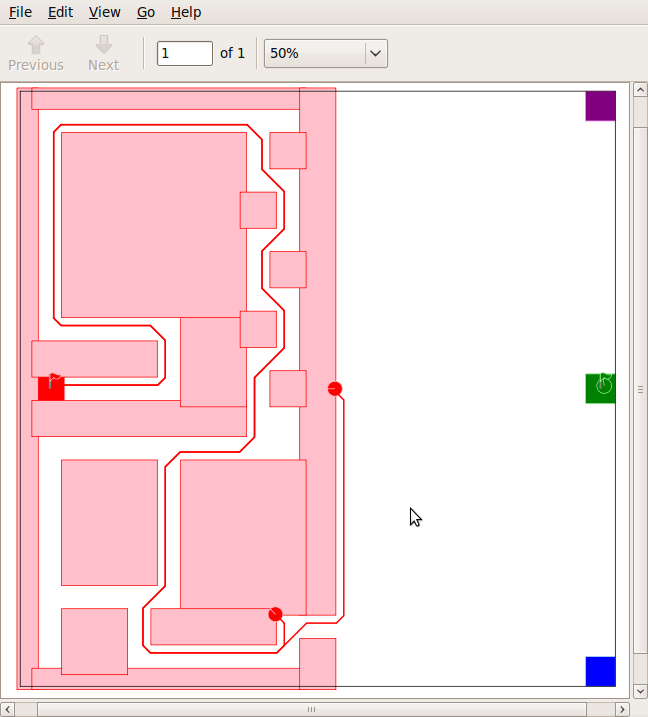
\includegraphics[width=\textwidth]{07re-evaluate-path.png}
\caption{Getting stuck at the wall on the way home. Re-evaluated path show}
\end{center}
\end{figure}
After we capture the flag the sniper agent is given the task to search for a path home, but always gets stuck against a wall and will remain stuck until the search path is re-evaluated. Once the path is re-evaluated we returned to home base successfully.  This is a problem we will need to fix in subsequent labs, but which did not stop us from passing this lab.

\subsection{Michael Hansen and Daniel Nelson}
We ran our tests with another group from class which consisted of:
\begin{itemize}
    \item{Michael Hansen}
    \item{Daniel Nelson}
\end{itemize}
What was interesting about watching the other team pass off was that they had a few problems in their implementation, but they were in no way related to the problems we encountered.  The main problem the other team had was that the decoy would get killed as it went into its decoy mode.  They had to change the timing of their agents to avoid this, but in the end they successfully completed the challenge.